% generated by scripts/pkl_to_latex.py
% source PKL : tscan_v1_L6_Ne4_U10_mode-uniform_nmin2_solver-gcg_full_restarts10_iter300_kmax4_tol1em09_t0.05to2_N20-d03538a42051.pkl
% scan type  : tscan
% state      : gs
% requires   : \usepackage{pgfplots} \pgfplotsset{compat=1.18}
% colours match the matplotlib PDF (tab10 cycle)
\definecolor{gmeC0}{HTML}{1F77B4}
\definecolor{gmeC1}{HTML}{FF7F0E}
\definecolor{gmeC2}{HTML}{2CA02C}
\definecolor{gmeC3}{HTML}{D62728}
\definecolor{gmeC4}{HTML}{9467BD}
\definecolor{gmeC5}{HTML}{8C564B}
\definecolor{gmeC6}{HTML}{E377C2}
\definecolor{gmeC7}{HTML}{17BECF}

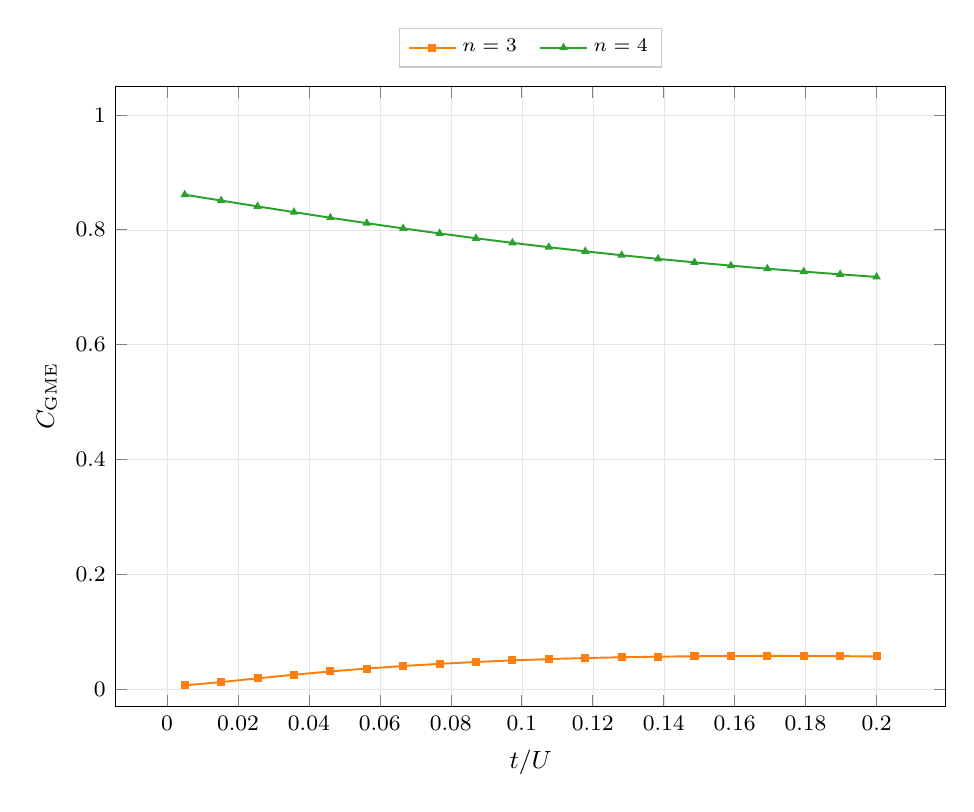
\begin{tikzpicture}
  \begin{axis}[
    width=\columnwidth,
    height=0.78\columnwidth,
    xlabel={$t/U$},
    ylabel={$C_{\mathrm{GME}}$},
    grid=both,
    grid style={line width=.1pt, draw=gray!20},
    tick label style={font=\footnotesize\rmfamily, /pgf/number format/fixed},
    label style={font=\small\rmfamily},
    scaled ticks=false,
    legend style={font=\scriptsize\rmfamily, draw=gray!40, at={(0.5,1.03)}, anchor=south, /tikz/every even column/.append style={column sep=6pt}},
    legend cell align={left},
    legend columns=2,
    ymin=-0.03,
    ymax=1.05,
  ]
    \addplot[color=gmeC1, mark=square*, mark size=1.1pt, line width=0.7pt] coordinates {
        (0.005,0.006649) (0.015263,0.012136) (0.025526,0.018722) (0.035789,0.025063)
        (0.046053,0.030746) (0.056316,0.035783) (0.066579,0.040196) (0.076842,0.044015)
        (0.087105,0.047274) (0.097368,0.05001) (0.107632,0.052262) (0.117895,0.054069)
        (0.128158,0.055471) (0.138421,0.056506) (0.148684,0.05721) (0.158947,0.057619)
        (0.169211,0.057766) (0.179474,0.05768) (0.189737,0.057391) (0.2,0.056923)
    };
    \addlegendentry{$n=3$}
    \addplot[color=gmeC2, mark=triangle*, mark size=1.1pt, line width=0.7pt] coordinates {
        (0.005,0.861022) (0.015263,0.850768) (0.025526,0.840604) (0.035789,0.830609)
        (0.046053,0.820851) (0.056316,0.811383) (0.066579,0.802251) (0.076842,0.793485)
        (0.087105,0.785106) (0.097368,0.777126) (0.107632,0.769549) (0.117895,0.762372)
        (0.128158,0.755586) (0.138421,0.749181) (0.148684,0.743141) (0.158947,0.73745)
        (0.169211,0.732091) (0.179474,0.727044) (0.189737,0.722292) (0.2,0.717816)
    };
    \addlegendentry{$n=4$}
  \end{axis}
\end{tikzpicture}
